\documentclass[]{article}
\usepackage{lmodern}
\usepackage{amssymb,amsmath}
\usepackage{ifxetex,ifluatex}
\usepackage{fixltx2e} % provides \textsubscript
\ifnum 0\ifxetex 1\fi\ifluatex 1\fi=0 % if pdftex
  \usepackage[T1]{fontenc}
  \usepackage[utf8]{inputenc}
\else % if luatex or xelatex
  \ifxetex
    \usepackage{mathspec}
  \else
    \usepackage{fontspec}
  \fi
  \defaultfontfeatures{Ligatures=TeX,Scale=MatchLowercase}
\fi
% use upquote if available, for straight quotes in verbatim environments
\IfFileExists{upquote.sty}{\usepackage{upquote}}{}
% use microtype if available
\IfFileExists{microtype.sty}{%
\usepackage{microtype}
\UseMicrotypeSet[protrusion]{basicmath} % disable protrusion for tt fonts
}{}
\usepackage[margin=1in]{geometry}
\usepackage{hyperref}
\hypersetup{unicode=true,
            pdftitle={Maragra update: December 2018},
            pdfborder={0 0 0},
            breaklinks=true}
\urlstyle{same}  % don't use monospace font for urls
\usepackage{graphicx,grffile}
\makeatletter
\def\maxwidth{\ifdim\Gin@nat@width>\linewidth\linewidth\else\Gin@nat@width\fi}
\def\maxheight{\ifdim\Gin@nat@height>\textheight\textheight\else\Gin@nat@height\fi}
\makeatother
% Scale images if necessary, so that they will not overflow the page
% margins by default, and it is still possible to overwrite the defaults
% using explicit options in \includegraphics[width, height, ...]{}
\setkeys{Gin}{width=\maxwidth,height=\maxheight,keepaspectratio}
\IfFileExists{parskip.sty}{%
\usepackage{parskip}
}{% else
\setlength{\parindent}{0pt}
\setlength{\parskip}{6pt plus 2pt minus 1pt}
}
\setlength{\emergencystretch}{3em}  % prevent overfull lines
\providecommand{\tightlist}{%
  \setlength{\itemsep}{0pt}\setlength{\parskip}{0pt}}
\setcounter{secnumdepth}{0}
% Redefines (sub)paragraphs to behave more like sections
\ifx\paragraph\undefined\else
\let\oldparagraph\paragraph
\renewcommand{\paragraph}[1]{\oldparagraph{#1}\mbox{}}
\fi
\ifx\subparagraph\undefined\else
\let\oldsubparagraph\subparagraph
\renewcommand{\subparagraph}[1]{\oldsubparagraph{#1}\mbox{}}
\fi

%%% Use protect on footnotes to avoid problems with footnotes in titles
\let\rmarkdownfootnote\footnote%
\def\footnote{\protect\rmarkdownfootnote}

%%% Change title format to be more compact
\usepackage{titling}

% Create subtitle command for use in maketitle
\newcommand{\subtitle}[1]{
  \posttitle{
    \begin{center}\large#1\end{center}
    }
}

\setlength{\droptitle}{-2em}

  \title{Maragra update: December 2018}
    \pretitle{\vspace{\droptitle}\centering\huge}
  \posttitle{\par}
  \subtitle{Brew, Pradhan, Sicuri}
  \author{}
    \preauthor{}\postauthor{}
    \date{}
    \predate{}\postdate{}
  
\pagenumbering{gobble}
\usepackage{longtable}
\usepackage[utf8]{inputenc}
\usepackage{changepage}
\usepackage{graphicx}
\usepackage{multicol}
\usepackage{geometry}
\usepackage{fancyhdr}
\usepackage{color}
\usepackage{colortbl}
\usepackage{color}
\usepackage{hyperref}
% Font
\usepackage{fontspec}
\setmainfont{Swift-Regular_43151.ttf}
\setsansfont[BoldFont={Swift-Bold_43130.ttf}]{Swift-Regular_43151.ttf}
% \setmonofont{Swift-Regular_43151.ttf}
\renewcommand{\familydefault}{\sfdefault}
% \usepackage{fontspec}
% \setmainfont{Lato-Regular.ttf}
% \setsansfont[BoldFont={Lato-Bold.ttf}]{Lato-Regular.ttf}
% \renewcommand{\familydefault}{\sfdefault}

\def\changemargin#1#2{\list{}{\rightmargin#2\leftmargin#1}\item[]}
\let\endchangemargin=\endlist
\renewcommand{\rmdefault}{ppl}

\usepackage{multicol}
\usepackage{hyperref}
\usepackage{geometry}
\usepackage{lipsum}

\usepackage{longtable}


\usepackage{float}
\floatplacement{figure}{H}

% \usepackage{todonotes} % for side notes
% \usepackage[colorinlistoftodos]{todonotes} % for side notes

\usepackage{xargs}                      % Use more than one optional parameter in a new commands
\usepackage[dvipsnames, table]{xcolor}  % Coloured text etc.
% 
\usepackage[colorinlistoftodos,prependcaption,textsize=tiny]{todonotes}
\newcommandx{\unsure}[2][1=]{\todo[linecolor=red,backgroundcolor=red!25,bordercolor=red,#1]{#2}}
\newcommandx{\change}[2][1=]{\todo[linecolor=blue,backgroundcolor=blue!25,bordercolor=blue,#1]{#2}}
\newcommandx{\info}[2][1=]{\todo[linecolor=OliveGreen,backgroundcolor=OliveGreen!25,bordercolor=OliveGreen,#1]{#2}}
\newcommandx{\improvement}[2][1=]{\todo[linecolor=Plum,backgroundcolor=Plum!25,bordercolor=Plum,#1]{#2}}
\newcommandx{\thiswillnotshow}[2][1=]{\todo[disable,#1]{#2}}
\usepackage{lmodern}
\usepackage{fancyhdr} % Headers and footers
\pagestyle{fancy} % All pages have headers and footers
\fancyhead{} % Blank out the default header
\fancyfoot{} % Blank out the default footer
\fancyhead[C]{Return on investment of private sector malaria control at a large sugar facility in Southern Mozambique}
\renewcommand{\thefootnote}{\fnsymbol{footnote}}

\newcommand{\footremember}[2]{%
    \footnote{#2}
    \newcounter{#1}
    \setcounter{#1}{\value{footnote}}%
}
\newcommand{\footrecall}[1]{%
    \footnotemark[\value{#1}]%
}

\def\changemargin#1#2{\list{}{\rightmargin#2\leftmargin#1}\item[]}
\let\endchangemargin=\endlist

\widowpenalties 1 150

\makeatletter
\renewcommand\footnotesize{%
   \@setfontsize\footnotesize\@ixpt{11}%
   \abovedisplayskip 8\p@ \@plus2\p@ \@minus4\p@
   \abovedisplayshortskip \z@ \@plus\p@
   \belowdisplayshortskip 4\p@ \@plus2\p@ \@minus2\p@
   \def\@listi{\leftmargin\leftmargini
               \topsep 4\p@ \@plus2\p@ \@minus2\p@
               \parsep 2\p@ \@plus\p@ \@minus\p@
               \itemsep \parsep}%
   \belowdisplayskip \abovedisplayskip
}
\makeatother

\DeclareTextCommandDefault{\nobreakspace}{\leavevmode\nobreak\ }
\usepackage{booktabs}
\usepackage{longtable}
\usepackage{array}
\usepackage{multirow}
\usepackage[table]{xcolor}
\usepackage{wrapfig}
\usepackage{float}
\usepackage{colortbl}
\usepackage{pdflscape}
\usepackage{tabu}
\usepackage{threeparttable}
\usepackage{threeparttablex}
\usepackage[normalem]{ulem}
\usepackage{makecell}

\begin{document}
\maketitle

\begin{center}
\begin{large}

Maragra models

\end{large}
\end{center}

\vspace{5mm}

\begin{center}
\textbf{Overview}  
\end{center}

\vspace{5mm}

\begin{center}
\begin{changemargin}{3cm}{3cm} 

This document contains an overview of the modeling approach and simulations results.

\end{changemargin}
\end{center}

\vspace{20mm}

\noindent\fbox{%
    \parbox{\textwidth}{%
        \subsection*{Main points}
        \begin{itemize}
          \item We have a new modeling approach
          \item We have carried out basic simulations for several malaria control strategies
          \item Results are consistent/coherent
          \item We have not yet implemented geographical variation
        \end{itemize}
        \vspace{2mm}
    }%
}

\vfill
\null

\subsection*{Desinataires}

\textbf{Elisa Sicuri; Menno Pradhan}

\vspace{3mm}

\newpage

\section{Current paper}\label{current-paper}

Draft of the paper
(\href{https://docs.google.com/document/d/1bUWRBCgVcgjSPHchIQxiTG8Vwv5hV1GLU4Tlu386sWA/edit#}{HERE}

\section{Code}\label{code}

In R, our model looks like this

\begin{verbatim}
felm(formula = log(absent + 1) ~ protection_var + (rain_var) | 
    oracle_number | 0 | 0, data = final_data)
\end{verbatim}

Where \texttt{protection} is the sum of all nearby IRS, weighted by the
inverse of the distance from the residence of the person (including the
person's own residence).

\newpage

\section{Reproduction of charts}\label{reproduction-of-charts}

\subsection{Number of workers by
department}\label{number-of-workers-by-department}

\begin{center}\includegraphics{nov2018_files/figure-latex/unnamed-chunk-4-1} \end{center}

\subsection{Number of temporary workers over
time}\label{number-of-temporary-workers-over-time}

\begin{center}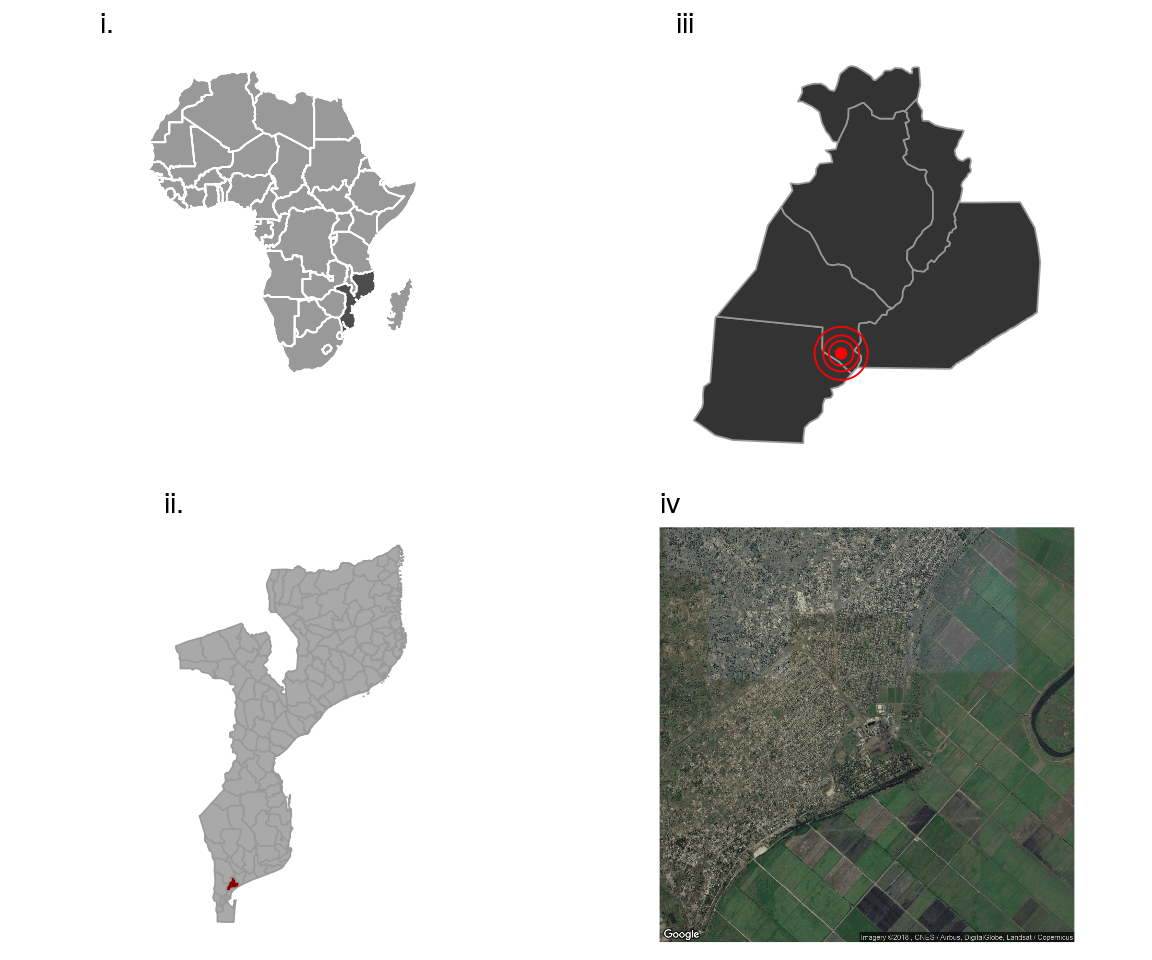
\includegraphics{nov2018_files/figure-latex/unnamed-chunk-5-1} \end{center}

\subsection{Absenteeism rate over
time}\label{absenteeism-rate-over-time}

\begin{center}\includegraphics{nov2018_files/figure-latex/unnamed-chunk-6-1} \end{center}

\subsection{Absenteeism rate over time by worker
type}\label{absenteeism-rate-over-time-by-worker-type}

\begin{center}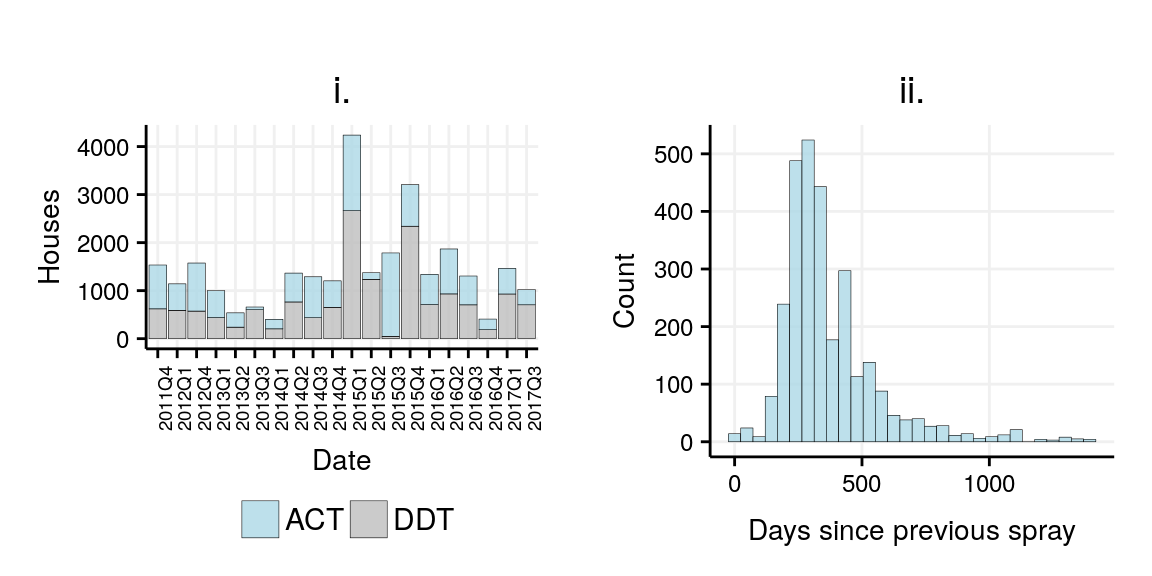
\includegraphics{nov2018_files/figure-latex/unnamed-chunk-7-1} \end{center}

\subsection{Number of workers over time by worker
type}\label{number-of-workers-over-time-by-worker-type}

\begin{center}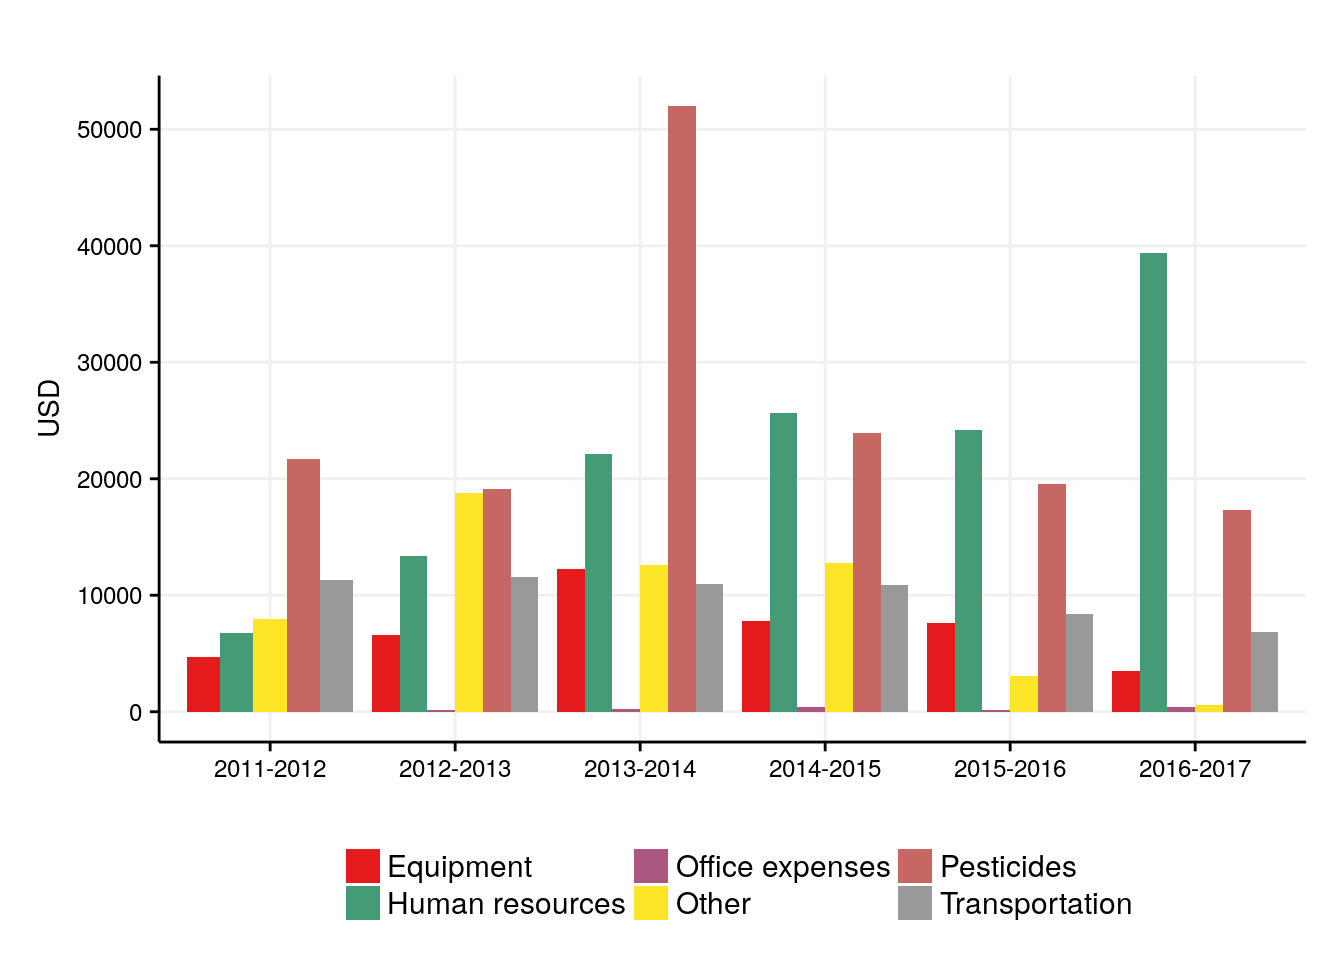
\includegraphics{nov2018_files/figure-latex/unnamed-chunk-8-1} \end{center}

\section{Descriptive overview}\label{descriptive-overview}

\subsection{Herd-only protection
score}\label{herd-only-protection-score}

\begin{tabular}{l|r}
\hline
Quantile & Absenteeism rate\\
\hline
Protection 1 & 10.641401\\
\hline
Protection 2 & 8.289246\\
\hline
Protection 3 & 8.312732\\
\hline
Protection 4 & 8.360836\\
\hline
\end{tabular}

\begin{center}\includegraphics{nov2018_files/figure-latex/unnamed-chunk-10-1} \end{center}

\newpage

\subsection{Individual-only protection
score}\label{individual-only-protection-score}

\begin{tabular}{l|r}
\hline
Quantile & Absenteeism rate\\
\hline
Protection 1 & 9.443294\\
\hline
Protection 2 & 8.464487\\
\hline
Protection 3 & 7.748320\\
\hline
Protection 4 & 7.792721\\
\hline
\end{tabular}

\begin{center}\includegraphics{nov2018_files/figure-latex/unnamed-chunk-12-1} \end{center}

\newpage

\subsection{Overall protection score}\label{overall-protection-score}

\begin{tabular}{l|l|r}
\hline
Quantile & Group & Absenteeism rate\\
\hline
Protection 1 & Permanent field worker & 13.687257\\
\hline
Protection 1 & Permanent not field worker & 11.415405\\
\hline
Protection 1 & Temporary field worker & 1.195219\\
\hline
Protection 1 & Temporary not field worker & 4.902265\\
\hline
Protection 2 & Permanent field worker & 11.210093\\
\hline
Protection 2 & Permanent not field worker & 10.136308\\
\hline
Protection 2 & Temporary field worker & 3.032894\\
\hline
Protection 2 & Temporary not field worker & 8.722060\\
\hline
Protection 3 & Permanent field worker & 10.542001\\
\hline
Protection 3 & Permanent not field worker & 10.447119\\
\hline
Protection 3 & Temporary field worker & 3.660856\\
\hline
Protection 3 & Temporary not field worker & 7.699303\\
\hline
Protection 4 & Permanent field worker & 11.371741\\
\hline
Protection 4 & Permanent not field worker & 10.374719\\
\hline
Protection 4 & Temporary field worker & 3.824707\\
\hline
Protection 4 & Temporary not field worker & 7.565523\\
\hline
\end{tabular}

\begin{center}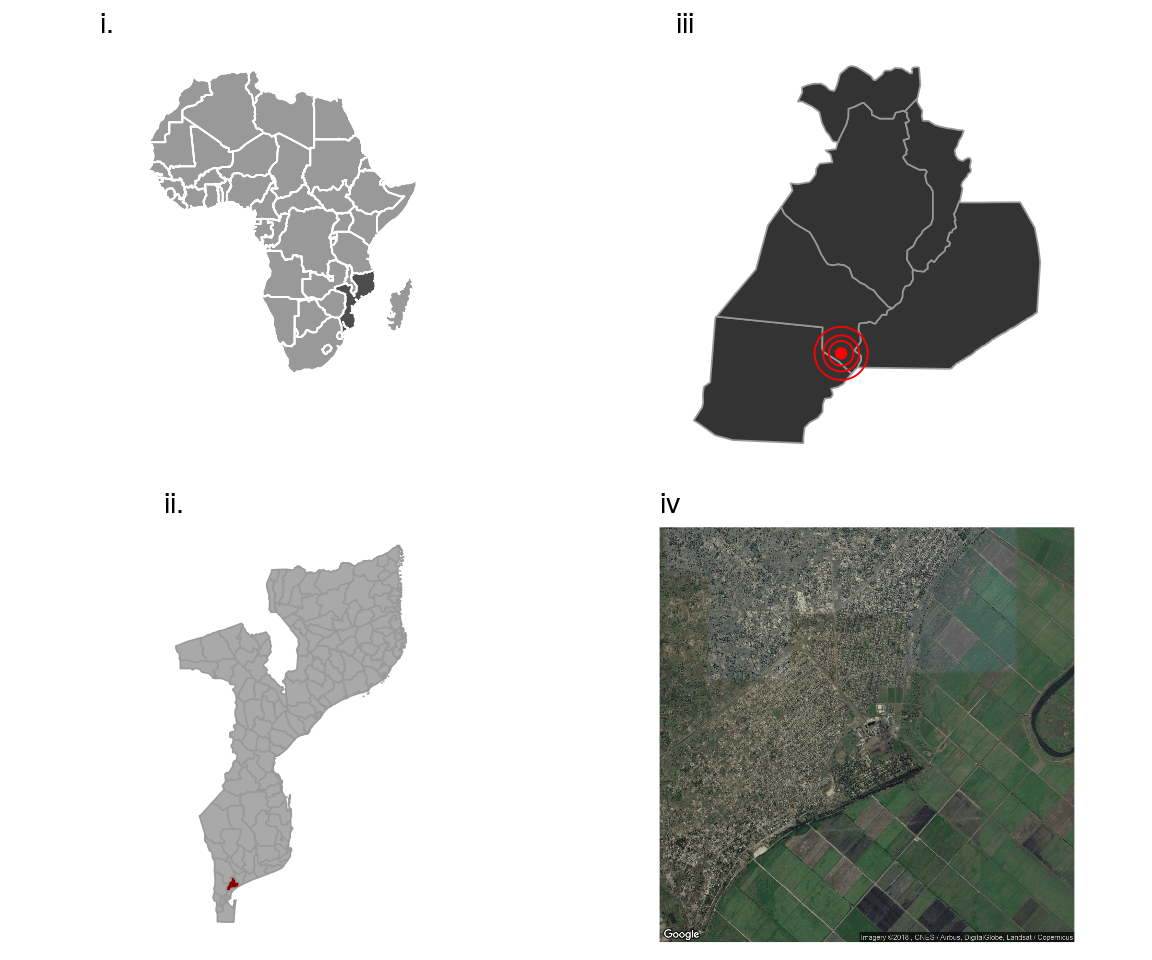
\includegraphics{nov2018_files/figure-latex/unnamed-chunk-14-1} \end{center}

\newpage

\subsection{Precipitation lag}\label{precipitation-lag}

\begin{tabular}{l|l|r}
\hline
Quantile & Group & Absenteeism rate\\
\hline
Protection 1 & Permanent field worker & 8.630077\\
\hline
Protection 1 & Permanent not field worker & 8.295415\\
\hline
Protection 1 & Temporary field worker & 3.535996\\
\hline
Protection 1 & Temporary not field worker & 7.870018\\
\hline
Protection 2 & Permanent field worker & 8.811771\\
\hline
Protection 2 & Permanent not field worker & 7.021752\\
\hline
Protection 2 & Temporary field worker & 3.439914\\
\hline
Protection 2 & Temporary not field worker & 7.246022\\
\hline
Protection 3 & Permanent field worker & 11.562734\\
\hline
Protection 3 & Permanent not field worker & 16.734109\\
\hline
Protection 3 & Temporary field worker & 3.099666\\
\hline
Protection 3 & Temporary not field worker & 5.810022\\
\hline
Protection 4 & Permanent field worker & 16.178230\\
\hline
Protection 4 & Permanent not field worker & 10.843800\\
\hline
Protection 4 & Temporary field worker & 2.916452\\
\hline
Protection 4 & Temporary not field worker & 9.779668\\
\hline
\end{tabular}

\begin{center}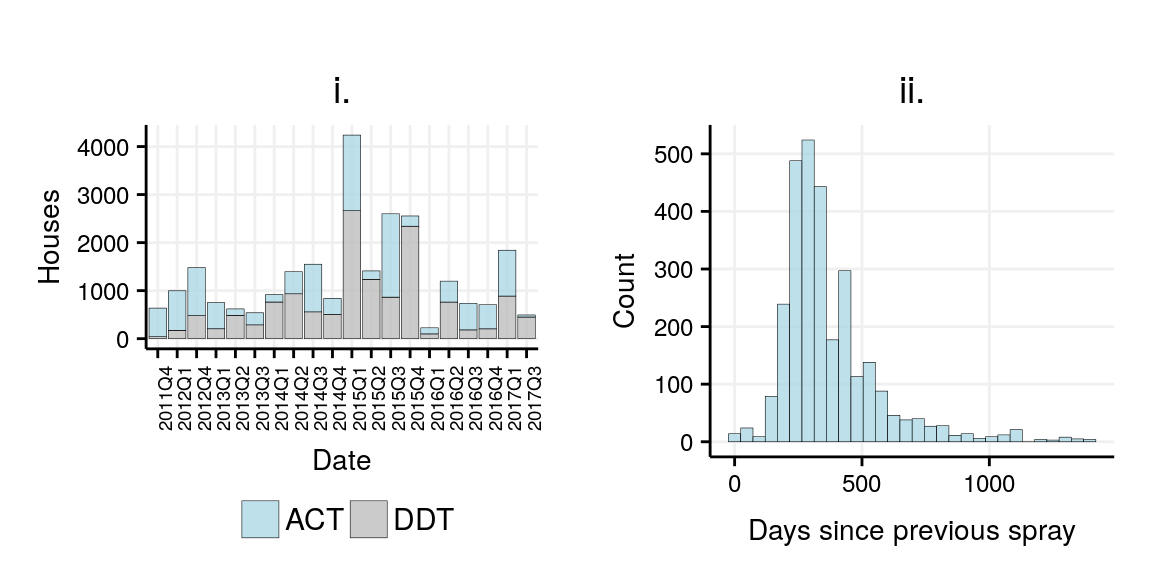
\includegraphics{nov2018_files/figure-latex/unnamed-chunk-16-1} \end{center}

\newpage

\section{Results}\label{results}

\subsection{Regression table}\label{regression-table}

The below table shows the results of the model devised thus far.

\begin{verbatim}

Call:
   felm(formula = log(absent + 1) ~ protection_var + (rain_var) |      oracle_number | 0 | 0, data = final_data) 

Residuals:
     Min       1Q   Median       3Q      Max 
-0.43174 -0.07695 -0.05705 -0.01099  0.69903 

Coefficients:
                 Estimate Std. Error t value Pr(>|t|)    
protection_var -4.462e-05  4.895e-06  -9.116   <2e-16 ***
rain_var        2.993e-03  2.042e-04  14.659   <2e-16 ***
---
Signif. codes:  0 '***' 0.001 '**' 0.01 '*' 0.05 '.' 0.1 ' ' 1

Residual standard error: 0.1916 on 308342 degrees of freedom
  (14642 observations deleted due to missingness)
Multiple R-squared(full model): 0.05462   Adjusted R-squared: 0.05273 
Multiple R-squared(proj model): 0.001288   Adjusted R-squared: -0.0007107 
F-statistic(full model):28.87 on 617 and 308342 DF, p-value: < 2.2e-16 
F-statistic(proj model): 198.8 on 2 and 308342 DF, p-value: < 2.2e-16 
\end{verbatim}

\subsection{Intepretation}\label{intepretation}

The below charts show predicted absenteeism rates at different rain and
protection levels.

\subsubsection{Precipitation's effect}\label{precipitations-effect}

\begin{center}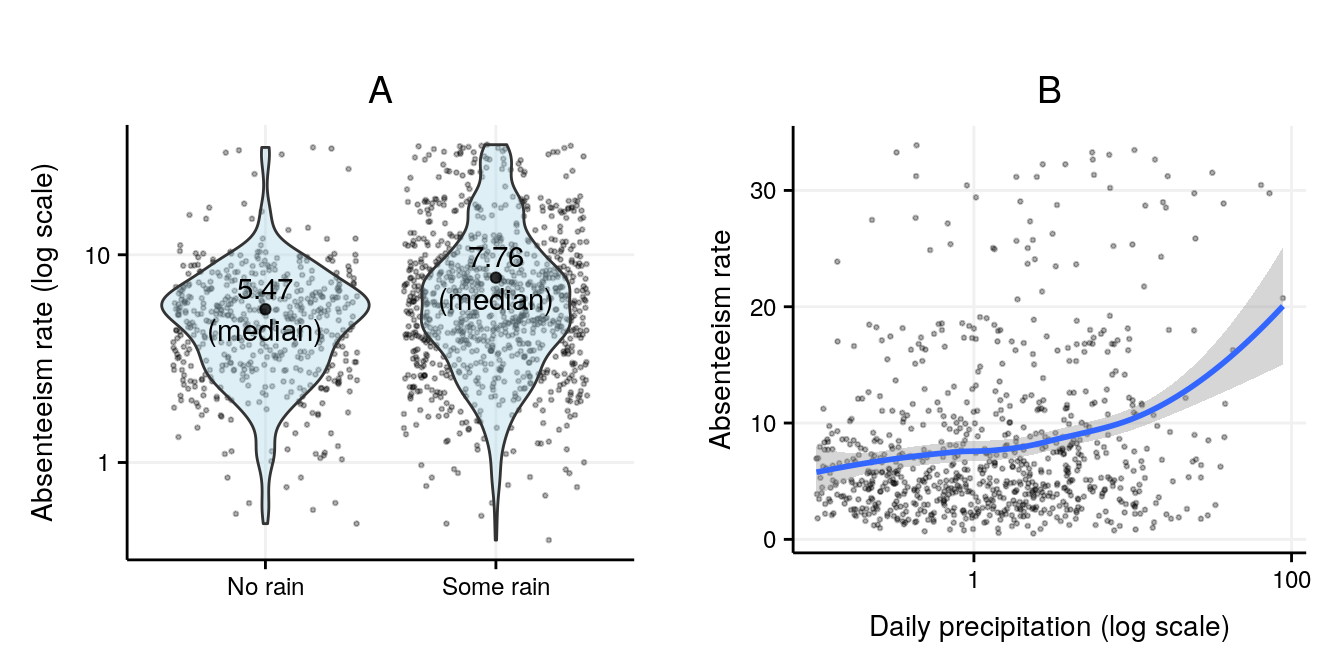
\includegraphics{nov2018_files/figure-latex/unnamed-chunk-20-1} \end{center}

\subsubsection{IRS protection's effect}\label{irs-protections-effect}

\begin{center}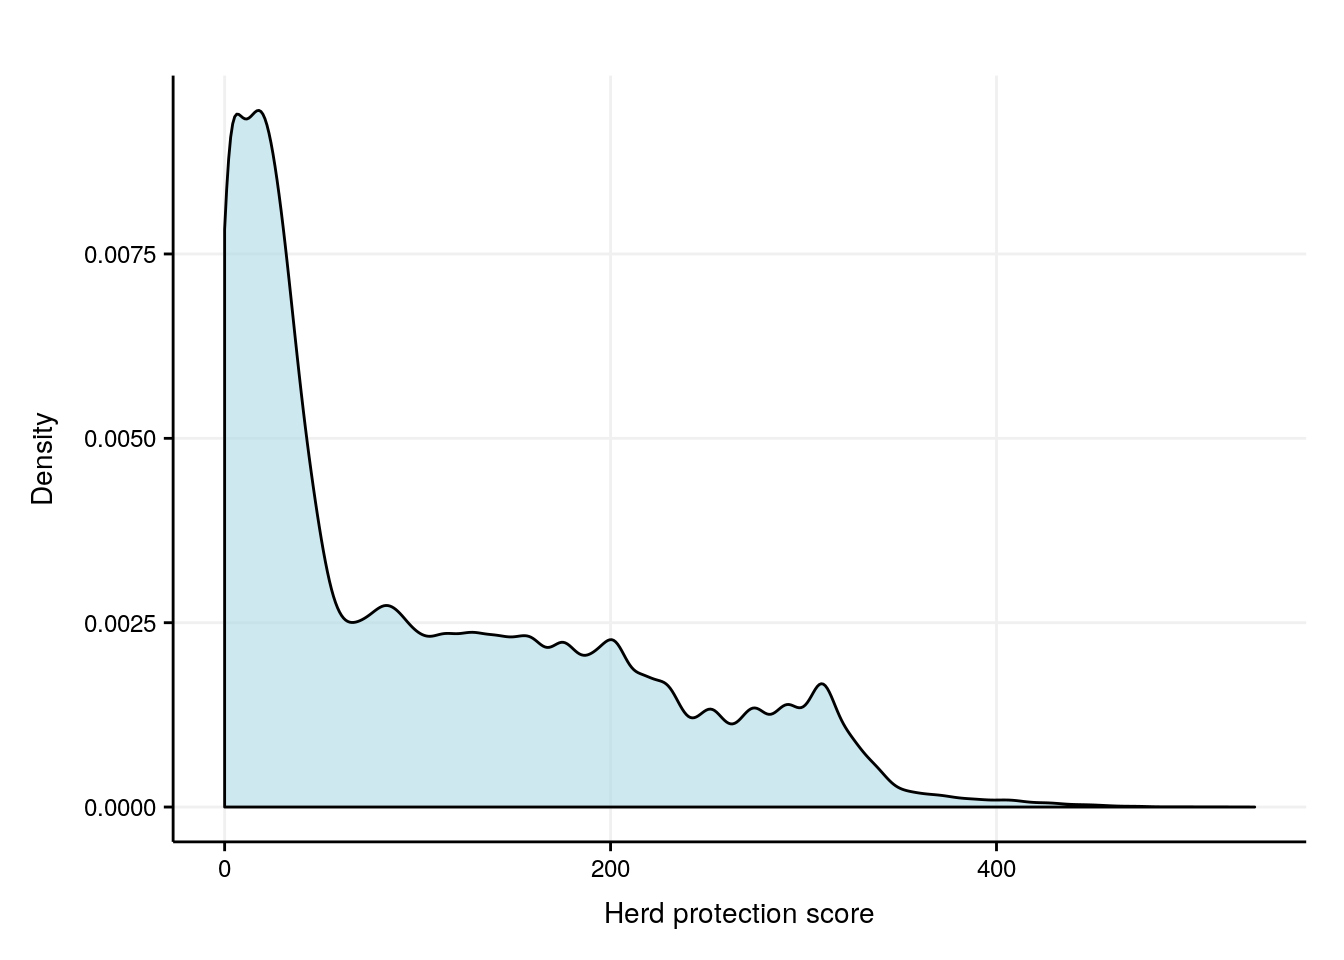
\includegraphics{nov2018_files/figure-latex/unnamed-chunk-21-1} \end{center}

\subsubsection{Simulations}\label{simulations}

\begin{tabular}{l|r|r}
\hline
strategy & value & predicted\_absences\\
\hline
Max & 0.1131433 & 34956.76\\
\hline
Real & 0.1250412 & 38632.73\\
\hline
Time-optimized & 0.1267574 & 39162.97\\
\hline
Zero & 0.1308765 & 40435.61\\
\hline
\end{tabular}

\begin{center}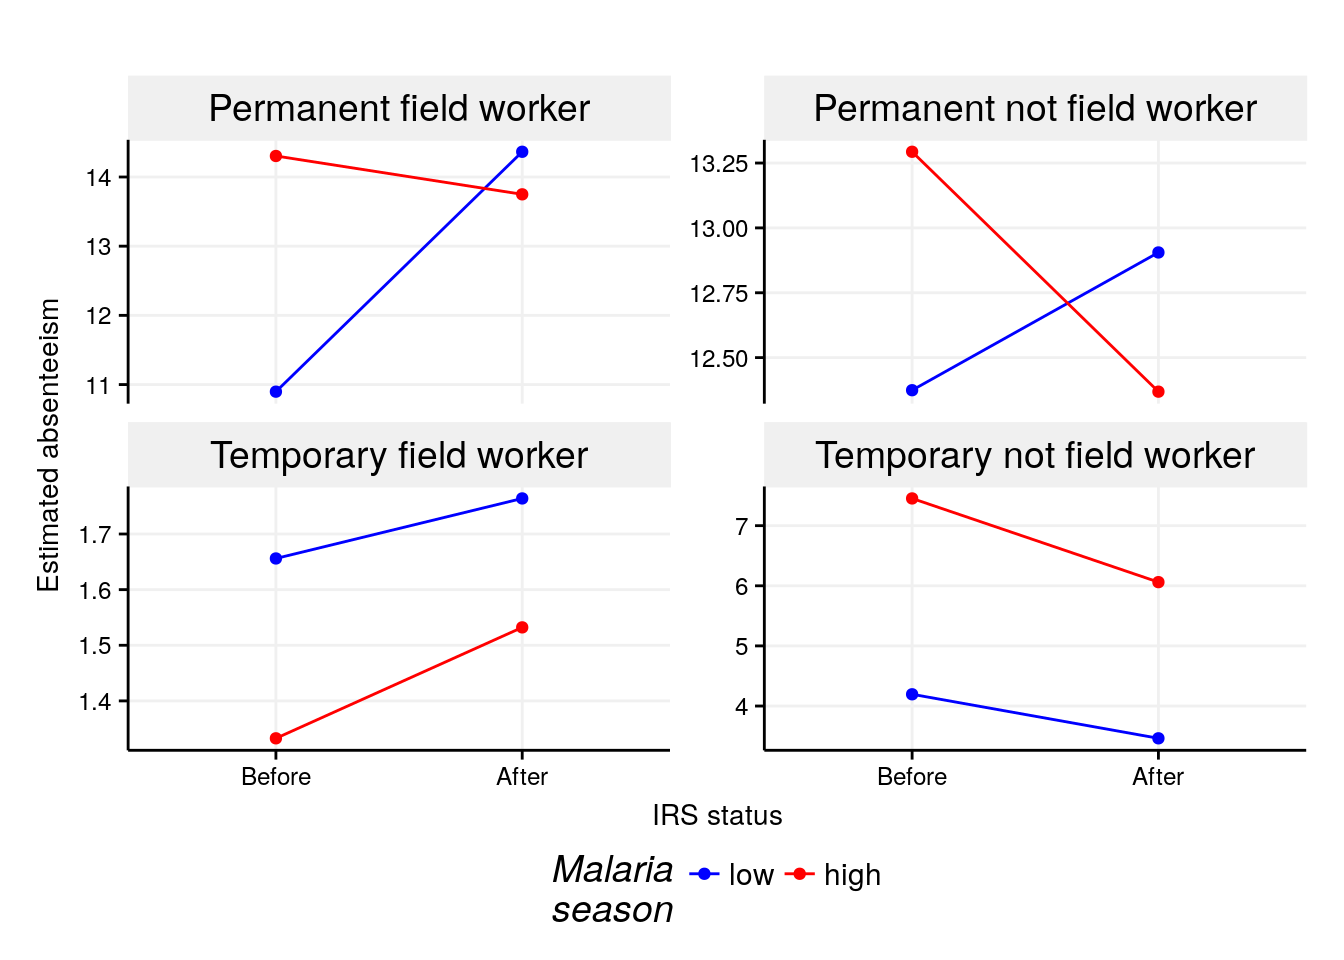
\includegraphics{nov2018_files/figure-latex/unnamed-chunk-23-1} \end{center}

\begin{center}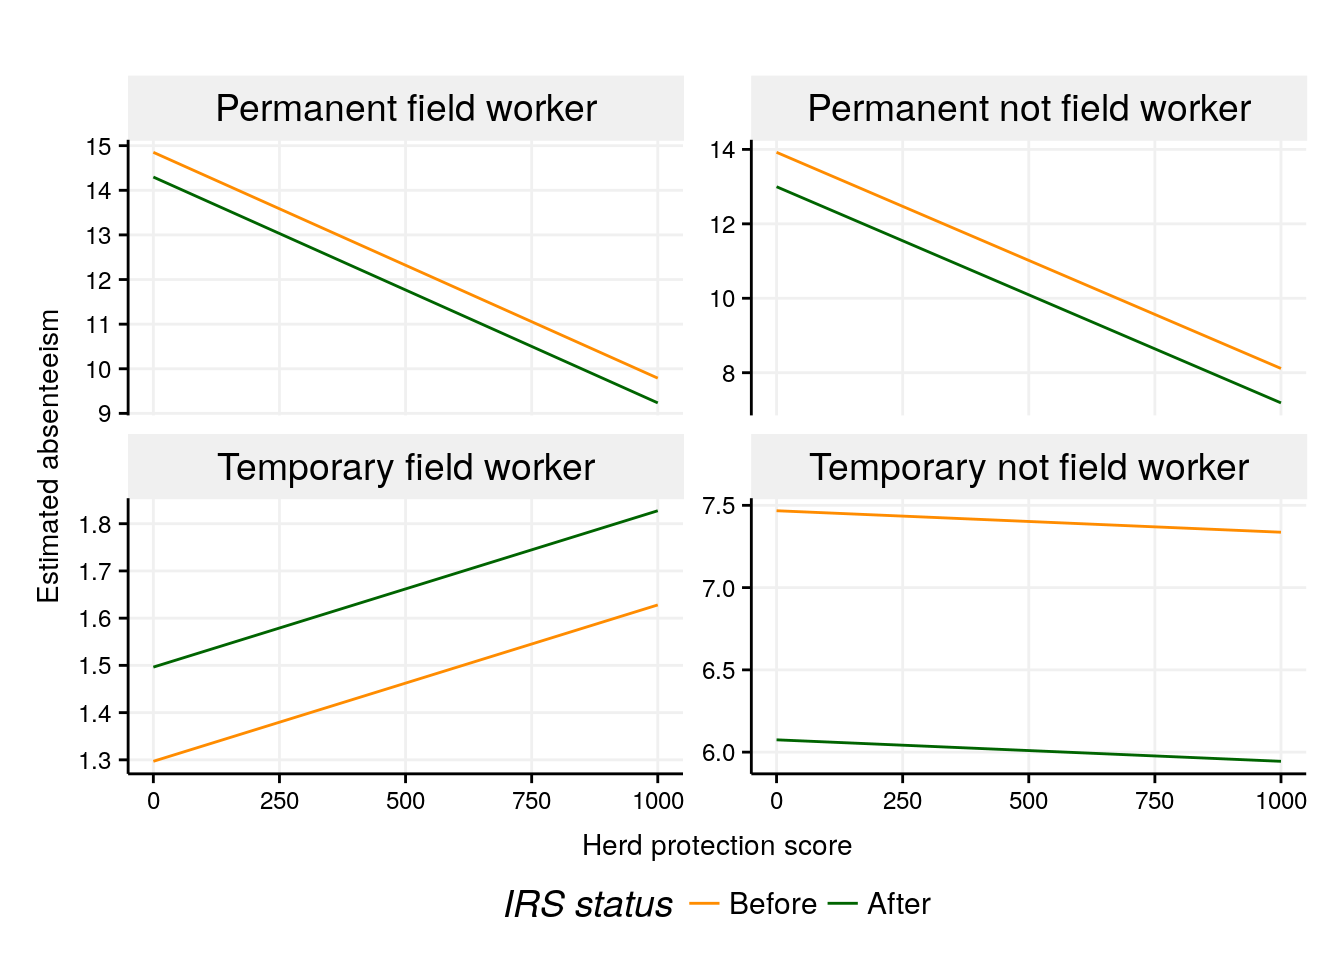
\includegraphics{nov2018_files/figure-latex/unnamed-chunk-24-1} \end{center}

\section{Costs}\label{costs}

\begin{tabular}{l|r}
\hline
strategy & sprays\\
\hline
Max & 8.520326\\
\hline
Real & 1.402844\\
\hline
Time-optimized & 1.507109\\
\hline
Zero & 0.000000\\
\hline
\end{tabular}

\begin{center}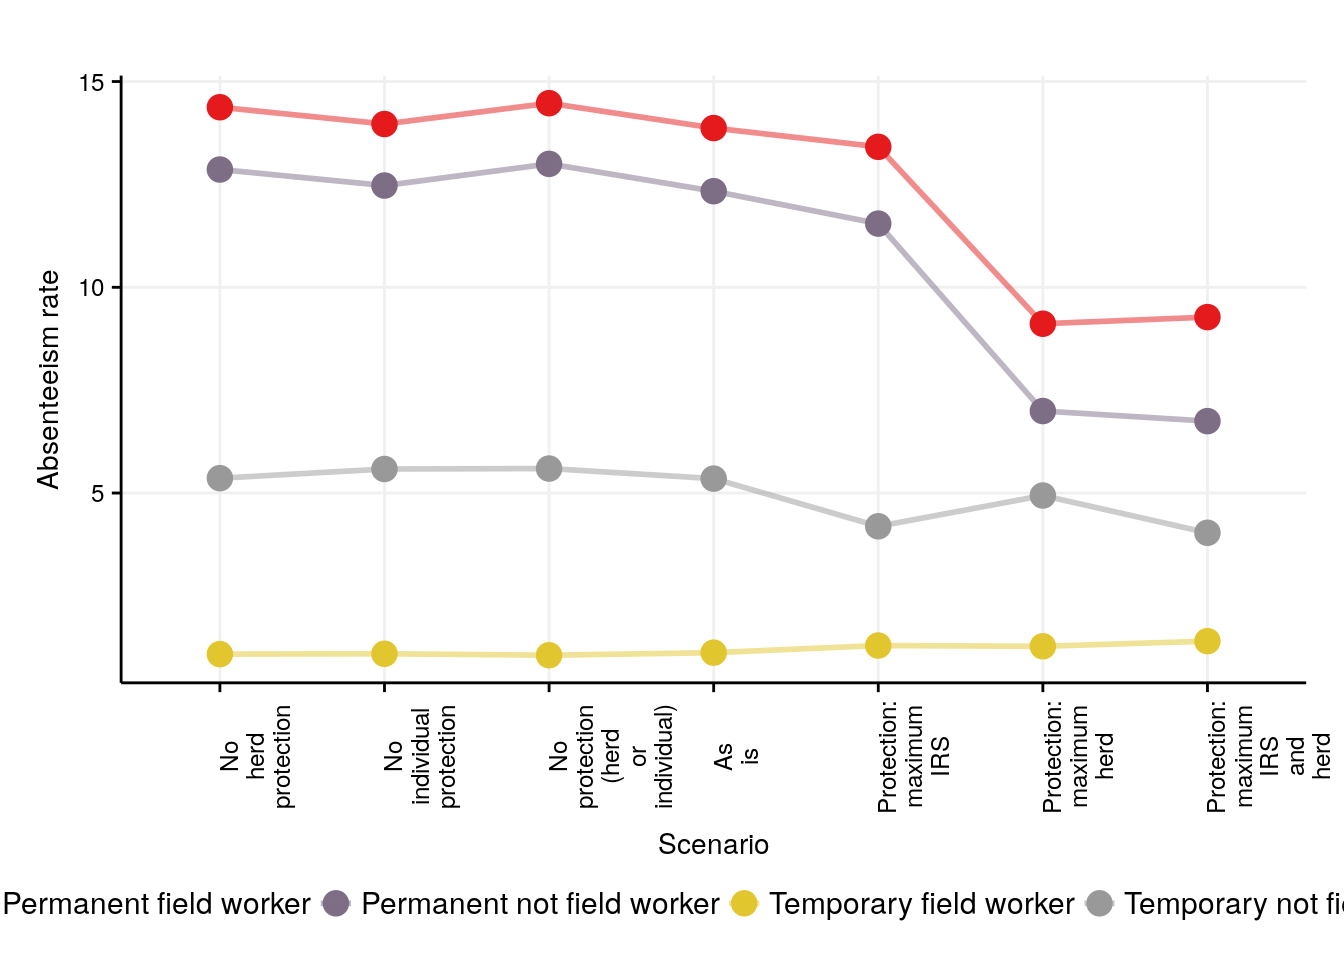
\includegraphics{nov2018_files/figure-latex/unnamed-chunk-25-1} \end{center}

\section{Bibliography}\label{bibliography}


\end{document}
